% Options for packages loaded elsewhere
\PassOptionsToPackage{unicode}{hyperref}
\PassOptionsToPackage{hyphens}{url}
%
\documentclass[
]{article}
\usepackage{lmodern}
\usepackage{amssymb,amsmath}
\usepackage{ifxetex,ifluatex}
\ifnum 0\ifxetex 1\fi\ifluatex 1\fi=0 % if pdftex
  \usepackage[T1]{fontenc}
  \usepackage[utf8]{inputenc}
  \usepackage{textcomp} % provide euro and other symbols
\else % if luatex or xetex
  \usepackage{unicode-math}
  \defaultfontfeatures{Scale=MatchLowercase}
  \defaultfontfeatures[\rmfamily]{Ligatures=TeX,Scale=1}
\fi
% Use upquote if available, for straight quotes in verbatim environments
\IfFileExists{upquote.sty}{\usepackage{upquote}}{}
\IfFileExists{microtype.sty}{% use microtype if available
  \usepackage[]{microtype}
  \UseMicrotypeSet[protrusion]{basicmath} % disable protrusion for tt fonts
}{}
\makeatletter
\@ifundefined{KOMAClassName}{% if non-KOMA class
  \IfFileExists{parskip.sty}{%
    \usepackage{parskip}
  }{% else
    \setlength{\parindent}{0pt}
    \setlength{\parskip}{6pt plus 2pt minus 1pt}}
}{% if KOMA class
  \KOMAoptions{parskip=half}}
\makeatother
\usepackage{xcolor}
\IfFileExists{xurl.sty}{\usepackage{xurl}}{} % add URL line breaks if available
\IfFileExists{bookmark.sty}{\usepackage{bookmark}}{\usepackage{hyperref}}
\hypersetup{
  pdftitle={Ionotropic receptors as the driving force behind human synapse establishment},
  pdfauthor={Lucas H. Viscardi; Danilo O. Imparato; Maria Cátira Bortolini; Rodrigo J. S. Dalmolin},
  pdfkeywords={Evolution, Nervous system},
  hidelinks,
  pdfcreator={LaTeX via pandoc}}
\urlstyle{same} % disable monospaced font for URLs
\usepackage[margin=1in]{geometry}
\usepackage{color}
\usepackage{fancyvrb}
\newcommand{\VerbBar}{|}
\newcommand{\VERB}{\Verb[commandchars=\\\{\}]}
\DefineVerbatimEnvironment{Highlighting}{Verbatim}{commandchars=\\\{\}}
% Add ',fontsize=\small' for more characters per line
\usepackage{framed}
\definecolor{shadecolor}{RGB}{48,48,48}
\newenvironment{Shaded}{\begin{snugshade}}{\end{snugshade}}
\newcommand{\AlertTok}[1]{\textcolor[rgb]{1.00,0.81,0.69}{#1}}
\newcommand{\AnnotationTok}[1]{\textcolor[rgb]{0.50,0.62,0.50}{\textbf{#1}}}
\newcommand{\AttributeTok}[1]{\textcolor[rgb]{0.80,0.80,0.80}{#1}}
\newcommand{\BaseNTok}[1]{\textcolor[rgb]{0.86,0.64,0.64}{#1}}
\newcommand{\BuiltInTok}[1]{\textcolor[rgb]{0.80,0.80,0.80}{#1}}
\newcommand{\CharTok}[1]{\textcolor[rgb]{0.86,0.64,0.64}{#1}}
\newcommand{\CommentTok}[1]{\textcolor[rgb]{0.50,0.62,0.50}{#1}}
\newcommand{\CommentVarTok}[1]{\textcolor[rgb]{0.50,0.62,0.50}{\textbf{#1}}}
\newcommand{\ConstantTok}[1]{\textcolor[rgb]{0.86,0.64,0.64}{\textbf{#1}}}
\newcommand{\ControlFlowTok}[1]{\textcolor[rgb]{0.94,0.87,0.69}{#1}}
\newcommand{\DataTypeTok}[1]{\textcolor[rgb]{0.87,0.87,0.75}{#1}}
\newcommand{\DecValTok}[1]{\textcolor[rgb]{0.86,0.86,0.80}{#1}}
\newcommand{\DocumentationTok}[1]{\textcolor[rgb]{0.50,0.62,0.50}{#1}}
\newcommand{\ErrorTok}[1]{\textcolor[rgb]{0.76,0.75,0.62}{#1}}
\newcommand{\ExtensionTok}[1]{\textcolor[rgb]{0.80,0.80,0.80}{#1}}
\newcommand{\FloatTok}[1]{\textcolor[rgb]{0.75,0.75,0.82}{#1}}
\newcommand{\FunctionTok}[1]{\textcolor[rgb]{0.94,0.94,0.56}{#1}}
\newcommand{\ImportTok}[1]{\textcolor[rgb]{0.80,0.80,0.80}{#1}}
\newcommand{\InformationTok}[1]{\textcolor[rgb]{0.50,0.62,0.50}{\textbf{#1}}}
\newcommand{\KeywordTok}[1]{\textcolor[rgb]{0.94,0.87,0.69}{#1}}
\newcommand{\NormalTok}[1]{\textcolor[rgb]{0.80,0.80,0.80}{#1}}
\newcommand{\OperatorTok}[1]{\textcolor[rgb]{0.94,0.94,0.82}{#1}}
\newcommand{\OtherTok}[1]{\textcolor[rgb]{0.94,0.94,0.56}{#1}}
\newcommand{\PreprocessorTok}[1]{\textcolor[rgb]{1.00,0.81,0.69}{\textbf{#1}}}
\newcommand{\RegionMarkerTok}[1]{\textcolor[rgb]{0.80,0.80,0.80}{#1}}
\newcommand{\SpecialCharTok}[1]{\textcolor[rgb]{0.86,0.64,0.64}{#1}}
\newcommand{\SpecialStringTok}[1]{\textcolor[rgb]{0.80,0.58,0.58}{#1}}
\newcommand{\StringTok}[1]{\textcolor[rgb]{0.80,0.58,0.58}{#1}}
\newcommand{\VariableTok}[1]{\textcolor[rgb]{0.80,0.80,0.80}{#1}}
\newcommand{\VerbatimStringTok}[1]{\textcolor[rgb]{0.80,0.58,0.58}{#1}}
\newcommand{\WarningTok}[1]{\textcolor[rgb]{0.50,0.62,0.50}{\textbf{#1}}}
\usepackage{graphicx,grffile}
\makeatletter
\def\maxwidth{\ifdim\Gin@nat@width>\linewidth\linewidth\else\Gin@nat@width\fi}
\def\maxheight{\ifdim\Gin@nat@height>\textheight\textheight\else\Gin@nat@height\fi}
\makeatother
% Scale images if necessary, so that they will not overflow the page
% margins by default, and it is still possible to overwrite the defaults
% using explicit options in \includegraphics[width, height, ...]{}
\setkeys{Gin}{width=\maxwidth,height=\maxheight,keepaspectratio}
% Set default figure placement to htbp
\makeatletter
\def\fps@figure{htbp}
\makeatother
\setlength{\emergencystretch}{3em} % prevent overfull lines
\providecommand{\tightlist}{%
  \setlength{\itemsep}{0pt}\setlength{\parskip}{0pt}}
\setcounter{secnumdepth}{-\maxdimen} % remove section numbering
\usepackage{booktabs}
\usepackage{longtable}
\usepackage{array}
\usepackage{multirow}
\usepackage{wrapfig}
\usepackage{float}
\usepackage{colortbl}
\usepackage{pdflscape}
\usepackage{tabu}
\usepackage{threeparttable}
\usepackage{threeparttablex}
\usepackage[normalem]{ulem}
\usepackage{makecell}
\usepackage{xcolor}
\let\oldShaded\Shaded
\let\endoldShaded\endShaded
\renewenvironment{Shaded}{\scriptsize\oldShaded}{\endoldShaded}
\let\oldverbatim\verbatim
\let\endoldverbatim\endverbatim
\renewenvironment{verbatim}{\scriptsize\oldverbatim}{\endoldverbatim}
\usepackage{caption}
\captionsetup{justification=raggedright,singlelinecheck=false}
\captionsetup{margin={2pt,0pt}}
\floatplacement{figure}{H}

\title{Ionotropic receptors as the driving force behind human synapse
establishment}
\usepackage{etoolbox}
\makeatletter
\providecommand{\subtitle}[1]{% add subtitle to \maketitle
  \apptocmd{\@title}{\par {\large #1 \par}}{}{}
}
\makeatother
\subtitle{Supplementary Material}
\author{Lucas H. Viscardi \and Danilo O. Imparato \and Maria Cátira Bortolini \and Rodrigo J. S. Dalmolin}
\date{}

\begin{document}
\maketitle
\begin{abstract}
Model uncertainty and limited data are fundamental challenges to robust
management of human intervention in a natural system. These challenges
are acutely highlighted by concerns that many ecological systems may
contain tipping points, such as Allee population sizes. Before a
collapse, we do not know where the tipping points lie, if they exist at
all. Hence, we know neither a complete model of the system dynamics nor
do we have access to data in some large region of state-space where such
a tipping point might exist.
\end{abstract}

{
\setcounter{tocdepth}{3}
\tableofcontents
}
\hypertarget{project-structure}{%
\section{Project structure}\label{project-structure}}

This is the title page

\hypertarget{preprocessing}{%
\section{Preprocessing}\label{preprocessing}}

This topic refers mainly to data wrangling done before the actual
analysis with the intent of making it simpler.

\hypertarget{eukaryota-species-tree}{%
\subsection{Eukaryota species tree}\label{eukaryota-species-tree}}

We opted to use the TimeTree database in order to obtain an standardized
Eukaryota species tree. However, some species were not present in it, so
we devised a way to fill them in based on NCBI Taxonomy data.

\hypertarget{ncbi-taxonomy-tree}{%
\subsubsection{NCBI Taxonomy tree}\label{ncbi-taxonomy-tree}}

First we preprocess NCBI Taxonomy data to leave only STRING eukaryotes,
thus making the task easier. \texttt{}

\hypertarget{resources}{%
\paragraph{\texorpdfstring{\textbf{Resources}}{Resources}}\label{resources}}

\texttt{}\\

\begin{table}[H]

\caption{\label{tab:string_species}Lists all organisms in STRING v11.}
\begin{tabular}[t]{rllll>{\raggedright\arraybackslash}p{18em}}
\toprule
\multicolumn{6}{c}{\bgroup\fontsize{12}{14}\selectfont \cellcolor[HTML]{EEEEEE}{\ttfamily{\textbf{string\_species}}}\egroup{}} \\
\cmidrule(l{3pt}r{3pt}){1-6}
\# & Col. name & Col. type & Used? & Example & Description\\
\midrule
\rowcolor{gray!6}  1 & taxid & character & yes & 9606 & NCBI Taxonomy identifier\\
2 & string\_type & character & no & core & if the genome of this species is core or periphery\\
\rowcolor{gray!6}  3 & string\_name & character & yes & Homo sapiens & STRING species name\\
4 & ncbi\_official\_name & character & no & Homo sapiens & NCBI Taxonomy species name\\
\bottomrule
\multicolumn{6}{l}{\textbf{Location: } data-raw/download/species.v11.0.txt}\\
\multicolumn{6}{l}{\textbf{Source: } stringdb-static.org/download/species.v11.0.txt}\\
\end{tabular}
\end{table}
\begin{table}[H]

\caption{\label{tab:ncbi_merged_ids}Links outdated taxon IDs to corresponding new ones.}
\begin{tabular}[t]{rllll>{\raggedright\arraybackslash}p{18em}}
\toprule
\multicolumn{6}{c}{\bgroup\fontsize{12}{14}\selectfont \cellcolor[HTML]{EEEEEE}{\ttfamily{\textbf{ncbi\_merged\_ids}}}\egroup{}} \\
\cmidrule(l{3pt}r{3pt}){1-6}
\# & Col. name & Col. type & Used? & Example & Description\\
\midrule
\rowcolor{gray!6}  1 & taxid & character & yes & 140100 & id of node that has been merged\\
2 & new\_taxid & character & yes & 666 & id of node that is the result of merging\\
\bottomrule
\multicolumn{6}{l}{\textbf{Location: } data-raw/download/taxdump/merged.dmp}\\
\multicolumn{6}{l}{\textbf{Source: } ftp.ncbi.nlm.nih.gov/pub/taxonomy/taxdump.tar.gz}\\
\end{tabular}
\end{table}
\begin{table}[H]

\caption{\label{tab:ncbi_edgelist}Represents taxonomy nodes.}
\begin{tabular}[t]{rllll>{\raggedright\arraybackslash}p{18em}}
\toprule
\multicolumn{6}{c}{\bgroup\fontsize{12}{14}\selectfont \cellcolor[HTML]{EEEEEE}{\ttfamily{\textbf{ncbi\_edgelist}}}\egroup{}} \\
\cmidrule(l{3pt}r{3pt}){1-6}
\# & Col. name & Col. type & Used? & Example & Description\\
\midrule
\rowcolor{gray!6}  1 & taxid & character & yes & 2 & node id in NCBI taxonomy database\\
2 & parent\_taxid & character & yes & 131567 & parent node id in NCBI taxonomy database\\
\rowcolor{gray!6}  3 & rank & character & no & superkingdom & rank of this node\\
4 & ... & ... & no & ... & (too many unrelated fields)\\
\bottomrule
\multicolumn{6}{l}{\textbf{Location: } data-raw/download/taxdump/nodes.dmp}\\
\multicolumn{6}{l}{\textbf{Source: } ftp.ncbi.nlm.nih.gov/pub/taxonomy/taxdump.tar.gz}\\
\end{tabular}
\end{table}
\begin{table}[H]

\caption{\label{tab:ncbi_taxon_names}Links taxon IDs to actual species names.}
\begin{tabular}[t]{rllll>{\raggedright\arraybackslash}p{18em}}
\toprule
\multicolumn{6}{c}{\bgroup\fontsize{12}{14}\selectfont \cellcolor[HTML]{EEEEEE}{\ttfamily{\textbf{ncbi\_taxon\_names}}}\egroup{}} \\
\cmidrule(l{3pt}r{3pt}){1-6}
\# & Col. name & Col. type & Used? & Example & Description\\
\midrule
\rowcolor{gray!6}  1 & taxid & character & yes & 2 & the id of node associated with this name\\
2 & name & character & yes & Monera & name itself\\
\rowcolor{gray!6}  3 & unique\_name & character & no & Monera <bacteria> & the unique variant of this name if name not unique\\
4 & name\_class & character & yes & scientific name & type of name\\
\bottomrule
\multicolumn{6}{l}{\textbf{Location: } data-raw/download/taxdump/names.dmp}\\
\multicolumn{6}{l}{\textbf{Source: } ftp.ncbi.nlm.nih.gov/pub/taxonomy/taxdump.tar.gz}\\
\end{tabular}
\end{table}

\texttt{}

\hypertarget{updating-string-taxon-ids}{%
\paragraph{\texorpdfstring{\textbf{Updating STRING taxon
IDs}}{Updating STRING taxon IDs}}\label{updating-string-taxon-ids}}

\texttt{}\\
Some organisms taxon IDs are outdated in STRING. We must update them to
work with the most recent NCBI Taxonomy data.

\begin{Shaded}
\begin{Highlighting}[]
\NormalTok{string_species }\OperatorTok
\StringTok{  }\KeywordTok{left_join}\NormalTok{(ncbi_merged_ids) }\OperatorTok
\StringTok{  }\KeywordTok{mutate}\NormalTok{(}\DataTypeTok{new_taxid =} \KeywordTok{coalesce}\NormalTok{(new_taxid, taxid))}
\end{Highlighting}
\end{Shaded}

\hypertarget{creating-tree-graph}{%
\paragraph{\texorpdfstring{\textbf{Creating tree
graph}}{Creating tree graph}}\label{creating-tree-graph}}

\texttt{}\\
The first step is to create a directed graph representing the NCBI
Taxonomy tree.

\begin{Shaded}
\begin{Highlighting}[]
\CommentTok{# leaving only "scientific name" rows}
\NormalTok{ncbi_taxon_names }\OperatorTok
\StringTok{  }\KeywordTok{filter}\NormalTok{(type }\OperatorTok{==}\StringTok{ "scientific name"}\NormalTok{) }\OperatorTok
\StringTok{  }\KeywordTok{select}\NormalTok{(name, ncbi_name)}

\CommentTok{# finding Eukaryota taxid}
\NormalTok{eukaryota_taxon_id <-}\StringTok{ }\KeywordTok{subset}\NormalTok{(ncbi_taxon_names, ncbi_name }\OperatorTok{==}\StringTok{ "Eukaryota"}\NormalTok{, }\StringTok{"name"}\NormalTok{, }\DataTypeTok{drop =} \OtherTok{TRUE}\NormalTok{)}

\CommentTok{# creating graph}
\NormalTok{g <-}\StringTok{ }\KeywordTok{graph_from_data_frame}\NormalTok{(ncbi_edgelist[,}\DecValTok{2}\OperatorTok{:}\DecValTok{1}\NormalTok{], }\DataTypeTok{directed =} \OtherTok{TRUE}\NormalTok{, }\DataTypeTok{vertices =}\NormalTok{ ncbi_taxon_names)}

\CommentTok{# easing memory}
\KeywordTok{rm}\NormalTok{(ncbi_edgelist, ncbi_merged_ids)}
\end{Highlighting}
\end{Shaded}

\hypertarget{traversing-the-graph}{%
\paragraph{\texorpdfstring{\textbf{Traversing the
graph}}{Traversing the graph}}\label{traversing-the-graph}}

\texttt{}\\
The second step is to traverse the graph from the Eukaryota root node to
STRING species nodes. This automatically drops all non-eukaryotes and
results in a species tree representing only STRING eukaryotes (476).

\begin{Shaded}
\begin{Highlighting}[]
\NormalTok{eukaryote_root <-}\StringTok{ }\KeywordTok{V}\NormalTok{(g)[eukaryota_taxon_id]}
\NormalTok{eukaryote_leaves <-}\StringTok{ }\KeywordTok{V}\NormalTok{(g)[string_species[[}\StringTok{"new_taxid"}\NormalTok{]]]}

\CommentTok{# not_found <- subset(string_species, !new_taxid %in% ncbi_taxon_names$name)}

\NormalTok{eukaryote_paths <-}\StringTok{ }\KeywordTok{shortest_paths}\NormalTok{(g, }\DataTypeTok{from =}\NormalTok{ eukaryote_root, }\DataTypeTok{to =}\NormalTok{ eukaryote_leaves, }\DataTypeTok{mode =} \StringTok{"out"}\NormalTok{)}\OperatorTok{$}\NormalTok{vpath}

\NormalTok{eukaryote_vertices <-}\StringTok{ }\NormalTok{eukaryote_paths }\OperatorTok\StringTok{ }\NormalTok{unlist }\OperatorTok\StringTok{ }\NormalTok{unique}

\NormalTok{eukaryote_tree <-}\StringTok{ }\KeywordTok{induced_subgraph}\NormalTok{(g, eukaryote_vertices, }\DataTypeTok{impl =} \StringTok{"create_from_scratch"}\NormalTok{)}
\end{Highlighting}
\end{Shaded}

\hypertarget{saving}{%
\paragraph{\texorpdfstring{\textbf{Saving}}{Saving}}\label{saving}}

\texttt{}\\
Saving \texttt{ncbi\_tree} and \texttt{string\_eukaryotes} for package
use. These data files are documented by the package. We also create a
plain text file \texttt{476\_ncbi\_eukaryotes.txt} containing the
updated names of all 476 STRING eukaryotes. This file will be queried
against the TimeTree website.

\begin{Shaded}
\begin{Highlighting}[]
\NormalTok{ncbi_tree <-}\StringTok{ }\NormalTok{treeio}\OperatorTok{::}\KeywordTok{as.phylo}\NormalTok{(eukaryote_tree)}

\CommentTok{# plot(ncbi_tree %>% ape::ladderize(), type="cladogram")}

\NormalTok{string_eukaryotes <-}\StringTok{ }\NormalTok{string_species }\OperatorTok
\StringTok{  }\KeywordTok{filter}\NormalTok{(new_taxid }\OperatorTok\StringTok{ }\NormalTok{ncbi_tree}\OperatorTok{$}\NormalTok{tip.label) }\OperatorTok
\StringTok{  }\KeywordTok{inner_join}\NormalTok{(ncbi_taxon_names, }\DataTypeTok{by =} \KeywordTok{c}\NormalTok{(}\StringTok{"new_taxid"}\NormalTok{ =}\StringTok{ "name"}\NormalTok{))}

\KeywordTok{write}\NormalTok{(string_eukaryotes[[}\StringTok{"ncbi_name"}\NormalTok{]],}\StringTok{"476_ncbi_eukaryotes.txt"}\NormalTok{)}

\CommentTok{# usethis::use_data(ncbi_tree, overwrite = TRUE)}
\KeywordTok{write.tree}\NormalTok{(ncbi_tree, }\StringTok{"ncbi_tree.nwk"}\NormalTok{)}
\NormalTok{usethis}\OperatorTok{::}\KeywordTok{use_data}\NormalTok{(string_eukaryotes, }\DataTypeTok{overwrite =} \OtherTok{TRUE}\NormalTok{)}
\end{Highlighting}
\end{Shaded}

\begin{verbatim}
## <U+2714> Setting active project to 'C:/R/neuro'
## <U+2714> Saving 'string_eukaryotes' to 'data/string_eukaryotes.rda'
\end{verbatim}


\hypertarget{duplicated-genera}{%
\subsubsection{Duplicated Genera}\label{duplicated-genera}}

Some species from different kingdoms may share the same genus name.
These genera must be noted down because one of the ways we fill in
missing species is by looking at genera names.
\hypertarget{loading-data}{%
\paragraph{\texorpdfstring{\textbf{Loading
data}}{Loading data}}\label{loading-data}}

\texttt{}\\
See \hyperref[tab:ncbi_edgelist]{Table 3} and
\hyperref[tab:ncbi_taxon_names]{Table 4}.

\begin{Shaded}
\begin{Highlighting}[]
\NormalTok{taxid_rank <-}\StringTok{ }\KeywordTok{read_delim}\NormalTok{(}
  \StringTok{"download/taxdump/nodes.dmp"}\NormalTok{,}
  \DataTypeTok{skip =} \DecValTok{1}\NormalTok{,}
  \DataTypeTok{delim =} \StringTok{"|"}\NormalTok{,}
  \DataTypeTok{trim_ws =} \OtherTok{TRUE}\NormalTok{,}
  \DataTypeTok{col_names =} \KeywordTok{c}\NormalTok{(}\StringTok{"taxid"}\NormalTok{,}\StringTok{"rank"}\NormalTok{),}
  \DataTypeTok{col_types =} \StringTok{"c-c"}
\NormalTok{)}

\NormalTok{ncbi_taxon_names <-}\StringTok{ }\KeywordTok{read_delim}\NormalTok{(}
  \StringTok{"download/taxdump/names.dmp"}\NormalTok{,}
  \DataTypeTok{delim =} \StringTok{"|"}\NormalTok{,}
  \DataTypeTok{trim_ws =} \OtherTok{TRUE}\NormalTok{,}
  \DataTypeTok{col_names =} \KeywordTok{c}\NormalTok{(}\StringTok{"taxid"}\NormalTok{,}\StringTok{"ncbi_name"}\NormalTok{,}\StringTok{"type"}\NormalTok{),}
  \DataTypeTok{col_types =} \StringTok{"cc-c"}
\NormalTok{)}
\end{Highlighting}
\end{Shaded}

\hypertarget{finding-duplicated-genera}{%
\paragraph{\texorpdfstring{\textbf{Finding duplicated
genera}}{Finding duplicated genera}}\label{finding-duplicated-genera}}

\texttt{}

\begin{Shaded}
\begin{Highlighting}[]
\CommentTok{# keeping genera nodes}
\NormalTok{taxid_rank }\OperatorTok\StringTok{ }\KeywordTok{filter}\NormalTok{(rank }\OperatorTok{==}\StringTok{ "genus"}\NormalTok{)}

\CommentTok{# keeping scientific names}
\NormalTok{ncbi_taxon_names }\OperatorTok
\StringTok{  }\KeywordTok{filter}\NormalTok{(type }\OperatorTok{==}\StringTok{ "scientific name"}\NormalTok{) }\OperatorTok
\StringTok{  }\KeywordTok{select}\NormalTok{(taxid, ncbi_name) }\OperatorTok
\StringTok{  }\KeywordTok{inner_join}\NormalTok{(taxid_rank)}

\CommentTok{# extracting and saving duplicated values}
\NormalTok{duplicated_genera <-}\StringTok{ }\NormalTok{ncbi_taxon_names }\OperatorTok
\StringTok{  }\KeywordTok{pull}\NormalTok{(ncbi_name) }\OperatorTok
\StringTok{  }\KeywordTok{extract}\NormalTok{(}\KeywordTok{duplicated}\NormalTok{(.)) }\OperatorTok
\StringTok{  }\KeywordTok{write}\NormalTok{(}\StringTok{"duplicated_genera.txt"}\NormalTok{)}
\end{Highlighting}
\end{Shaded}



\hypertarget{hybrid-tree}{%
\subsubsection{Hybrid tree}\label{hybrid-tree}}

Once we have both the NCBI eukaryotes tree and the list of duplicated
genera, we can start assembling the complete hybrid tree.
\hypertarget{resources}{%
\paragraph{Resources}\label{resources}}

\texttt{}\\
Besides downloading all TimeTree species data
(\texttt{Eukaryota\_species.nwk}) we also need to manually query the
website for the 476 STRING eukaryotes
(\texttt{476\_ncbi\_eukaryotes.txt}). The file is called
\texttt{476\_ncbi\_eukaryotes.txt} because it contains updated NCBI
Taxonomy names rather than STRING outdated names. This ensures better
results.

\begin{Shaded}
\begin{Highlighting}[]
\KeywordTok{download_if_missing}\NormalTok{(}
  \KeywordTok{paste0}\NormalTok{(}\StringTok{"http://timetree.org/ajax/direct_download"}\NormalTok{,}
         \StringTok{"?direct-download-format=newick"}\NormalTok{,}
         \StringTok{"&direct-download-id=23070"}\NormalTok{,}
         \StringTok{"&direct-download-rank=species"}\NormalTok{),}
  \StringTok{"Eukaryota_species.nwk"}
\NormalTok{)}
\end{Highlighting}
\end{Shaded}

\texttt{timetree\_newick} is the tree obtained by manually uploading
\texttt{476\_ncbi\_eukaryotes.txt} to the TimeTree website.
\texttt{tree\_85k} is the complete Eukaryota tree we have just
downloaded.

\begin{Shaded}
\begin{Highlighting}[]
\CommentTok{# loading species names and taxon ids}
\KeywordTok{load}\NormalTok{(}\StringTok{"../data/string_eukaryotes.rda"}\NormalTok{)}

\CommentTok{# loading newick tree manually obtained from timetree}
\NormalTok{timetree_newick <-}\StringTok{ }\KeywordTok{read.tree}\NormalTok{(}\StringTok{"download/timetree_335_eukaryotes.nwk"}\NormalTok{)}

\CommentTok{# the following genera names are unreliable and should not be searched for}
\NormalTok{duplicated_genera <-}\StringTok{ }\KeywordTok{scan}\NormalTok{(}\StringTok{"duplicated_genera.txt"}\NormalTok{, }\DataTypeTok{what =} \StringTok{"character"}\NormalTok{)}

\CommentTok{# loading all TimeTree species data we have just download (85000 species)}
\NormalTok{tree_85k <-}\StringTok{ }\KeywordTok{read.tree}\NormalTok{(}\StringTok{"download/Eukaryota_species.nwk"}\NormalTok{)}
\end{Highlighting}
\end{Shaded}

\hypertarget{unfound-species-with-matching-genera}{%
\paragraph{\texorpdfstring{\textbf{Unfound species with matching
genera}}{Unfound species with matching genera}}\label{unfound-species-with-matching-genera}}

\texttt{}\\
Some of the 476 STRING eukaryotes are not present in the TimeTree
database. However, sometimes TimeTree does contain tree data for closely
related species (e.g.~\emph{Monosiga brevicollis} is not present, but
\emph{Monosiga ovata} is). Therefore, we can use these closely related
species as proxies for the actual species. This is done by searching for
genera names in the complete database (\texttt{Eukaryota\_species.nwk}).
In the given \emph{Monosiga brevicollis} example, we search for
\emph{Monosiga} in the complete database. We see that there is
information for at least one other species of the \emph{Monosiga} genus
(in this case, \emph{Monosiga ovata}), so we add \emph{Monosiga
brevicollis} as a sister branch to the found species.

When you search for a term in TimeTree, it uses a synonym list obtained
from NCBI to try to resolve it. Sometimes TimeTree will resolve a
searched term to a scientific name different from the one you searched
for. The problem with this is that TimeTree does not make it obvious
that it is returning a different term. The first step is to find out
which species resolved to different names in the
\texttt{timetree\_335\_eukaryotes.nwk} file:

\begin{Shaded}
\begin{Highlighting}[]
\CommentTok{# plot(timetree_newick %>% ladderize, type = "cladogram", use.edge.length = F)}

\CommentTok{# replacing timetree species underscores with spaces}
\NormalTok{timetree_newick[[}\StringTok{"tip.label"}\NormalTok{]] }\OperatorTok\StringTok{ }\KeywordTok{str_replace_all}\NormalTok{(}\StringTok{"_"}\NormalTok{, }\StringTok{" "}\NormalTok{)}

\CommentTok{# which timetree species' names exactly match with ncbi's}
\NormalTok{taxid_indexes <-}\StringTok{ }\NormalTok{timetree_newick[[}\StringTok{"tip.label"}\NormalTok{]] }\OperatorTok\StringTok{ }\KeywordTok{match}\NormalTok{(string_eukaryotes[[}\StringTok{"ncbi_name"}\NormalTok{]])}

\CommentTok{# find out which timetree species names didn't exactly match ncbi's}
\NormalTok{unmatched_names <-}\StringTok{ }\NormalTok{timetree_newick[[}\StringTok{"tip.label"}\NormalTok{]] }\OperatorTok\StringTok{ }\NormalTok{magrittr}\OperatorTok{::}\KeywordTok{extract}\NormalTok{(taxid_indexes }\OperatorTok\StringTok{ }\NormalTok{is.na)}
\KeywordTok{print}\NormalTok{(unmatched_names)}
\end{Highlighting}
\end{Shaded}

\begin{verbatim}
## [1] "Cercospora fijiensis"     "Arthroderma benhamiae"   
## [3] "Macropus eugenii"         "Ostreococcus lucimarinus"
## [5] "Oryza nivara"
\end{verbatim}

\begin{Shaded}
\begin{Highlighting}[]
\CommentTok{# manually creating lookup table to be joined}
\NormalTok{ncbi_to_timetree <-}\StringTok{ }\KeywordTok{tribble}\NormalTok{(}
  \OperatorTok{~}\NormalTok{timetree_name,              }\OperatorTok{~}\NormalTok{ncbi_name,}
  \StringTok{"Cercospora fijiensis"}\NormalTok{,      }\StringTok{"Pseudocercospora fijiensis"}\NormalTok{,}
  \StringTok{"Arthroderma benhamiae"}\NormalTok{,     }\StringTok{"Trichophyton benhamiae"}\NormalTok{,}
  \StringTok{"Macropus eugenii"}\NormalTok{,          }\StringTok{"Notamacropus eugenii"}\NormalTok{,}
  \StringTok{"Ostreococcus lucimarinus"}\NormalTok{,  }\StringTok{"Ostreococcus sp. 'lucimarinus'"}\NormalTok{,}
  \StringTok{"Oryza nivara"}\NormalTok{,              }\StringTok{"Oryza sativa f. spontanea"}
\NormalTok{)}

\CommentTok{# joining info}
\NormalTok{species_dictionary <-}\StringTok{ }\NormalTok{string_eukaryotes }\OperatorTok\StringTok{ }\KeywordTok{left_join}\NormalTok{(ncbi_to_timetree)}

\CommentTok{# coalescing NAs to ncbi_name}
\NormalTok{species_dictionary }\OperatorTok
\StringTok{  }\KeywordTok{mutate}\NormalTok{(}\DataTypeTok{timetree_name =} \KeywordTok{coalesce}\NormalTok{(timetree_name, ncbi_name)) }\OperatorTok
\StringTok{  }\KeywordTok{mutate}\NormalTok{(}\DataTypeTok{timetree_name =} \KeywordTok{ifelse}\NormalTok{(timetree_name }\OperatorTok\StringTok{ }\NormalTok{timetree_newick[[}\StringTok{"tip.label"}\NormalTok{]], timetree_name, }\OtherTok{NA}\NormalTok{))}
\end{Highlighting}
\end{Shaded}

Now we can start looking for unfound species genera in the complete tree
data.

\begin{Shaded}
\begin{Highlighting}[]
\CommentTok{# annotating genera}
\NormalTok{species_dictionary }\OperatorTok
\StringTok{  }\KeywordTok{mutate}\NormalTok{(}\DataTypeTok{genus_search =} \KeywordTok{coalesce}\NormalTok{(timetree_name, ncbi_name) }\OperatorTok
\StringTok{  }\KeywordTok{strsplit}\NormalTok{(}\StringTok{" "}\NormalTok{) }\OperatorTok
\StringTok{  }\KeywordTok{sapply}\NormalTok{(}\StringTok{"["}\NormalTok{, }\DecValTok{1}\NormalTok{))}

\CommentTok{# unique genera}
\NormalTok{selected_genera <-}\StringTok{ }\NormalTok{species_dictionary[[}\StringTok{"genus_search"}\NormalTok{]] }\OperatorTok\StringTok{ }\NormalTok{unique}

\CommentTok{# these are unreliable selected_genera:}
\NormalTok{unreliable_genera <-}\StringTok{ }\KeywordTok{intersect}\NormalTok{(selected_genera, duplicated_genera)}

\CommentTok{# ensuring a cleaner newick file with only necessary data}
\CommentTok{# this is actually really important}
\NormalTok{tree_85k[[}\StringTok{"node.label"}\NormalTok{]] <-}\StringTok{ }\OtherTok{NULL}
\NormalTok{tree_85k[[}\StringTok{"edge.length"}\NormalTok{]] <-}\StringTok{ }\OtherTok{NULL}

\CommentTok{# replacing timetree's underscores with spaces}
\NormalTok{tree_85k[[}\StringTok{"tip.label"}\NormalTok{]] }\OperatorTok\StringTok{ }\KeywordTok{str_replace_all}\NormalTok{(}\StringTok{"_"}\NormalTok{, }\StringTok{" "}\NormalTok{)}

\CommentTok{# storing genus}
\NormalTok{tree_85k[[}\StringTok{"tip.genus"}\NormalTok{]] <-}\StringTok{ }\KeywordTok{sapply}\NormalTok{(}\KeywordTok{strsplit}\NormalTok{(tree_85k[[}\StringTok{"tip.label"}\NormalTok{]],}\StringTok{" "}\NormalTok{), }\StringTok{"["}\NormalTok{, }\DecValTok{1}\NormalTok{)}
\NormalTok{tree_85k_genera <-}\StringTok{ }\NormalTok{tree_85k[[}\StringTok{"tip.genus"}\NormalTok{]] }\OperatorTok\StringTok{ }\NormalTok{unique}

\CommentTok{# subtracting unreliable genera}
\NormalTok{tree_85k_genera }\OperatorTok\StringTok{ }\KeywordTok{setdiff}\NormalTok{(unreliable_genera)}

\CommentTok{# keeping only selected genera, including unreliable ones}
\NormalTok{tree_genus <-}\StringTok{ }\NormalTok{tree_85k }\OperatorTok\StringTok{ }\KeywordTok{keep.tip}\NormalTok{(., tip.label[tip.genus }\OperatorTok\StringTok{ }\NormalTok{selected_genera])}
\NormalTok{tree_genus[[}\StringTok{"tip.genus"}\NormalTok{]] <-}\StringTok{ }\KeywordTok{sapply}\NormalTok{(}\KeywordTok{strsplit}\NormalTok{(tree_genus[[}\StringTok{"tip.label"}\NormalTok{]],}\StringTok{" "}\NormalTok{), }\StringTok{"["}\NormalTok{, }\DecValTok{1}\NormalTok{)}

\CommentTok{# unfound species which genera are present in the 85k tree}
\NormalTok{unfound_species <-}\StringTok{ }\NormalTok{species_dictionary }\OperatorTok
\StringTok{  }\KeywordTok{filter}\NormalTok{(}\KeywordTok{is.na}\NormalTok{(timetree_name) }\OperatorTok{&}\StringTok{ }\NormalTok{genus_search }\OperatorTok\StringTok{ }\NormalTok{tree_85k_genera)}
\end{Highlighting}
\end{Shaded}

Once we figured out which species have proxy genera in the complete
data, we can start filling them in as sister branches.

\begin{Shaded}
\begin{Highlighting}[]
\CommentTok{# for each unfound species which genus is present in the 85k tree,}
\ControlFlowTok{for}\NormalTok{(i }\ControlFlowTok{in} \DecValTok{1}\OperatorTok{:}\KeywordTok{nrow}\NormalTok{(unfound_species))\{}
  \CommentTok{# we search for all species of this genus ("sister species") in the 85k tree}
  \CommentTok{# this part is tricky because bind.tip rebuilds the tree from scratch}
  \CommentTok{# so we need to keep removing underscores. there are better ways to do this.}
\NormalTok{  tip_genus <-}\StringTok{ }\NormalTok{tree_genus[[}\StringTok{"tip.label"}\NormalTok{]] }\OperatorTok\StringTok{ }\KeywordTok{strsplit}\NormalTok{(}\StringTok{"[_ ]"}\NormalTok{) }\OperatorTok\StringTok{ }\KeywordTok{sapply}\NormalTok{(}\StringTok{"["}\NormalTok{, }\DecValTok{1}\NormalTok{)}
\NormalTok{  sister_species <-}\StringTok{ }\NormalTok{tree_genus[[}\StringTok{"tip.label"}\NormalTok{]][tip_genus }\OperatorTok{==}\StringTok{ }\NormalTok{unfound_species[[i, }\StringTok{"genus_search"}\NormalTok{]]]}
  \CommentTok{# we obtain the sister_species' most recent common ancestor (MRCA)}
  \CommentTok{# c(.[1]) is a hack because the MRCA function only works with at least 2 nodes}
\NormalTok{  where <-}\StringTok{ }\KeywordTok{getMRCA}\NormalTok{(tree_genus, sister_species }\OperatorTok\StringTok{ }\KeywordTok{c}\NormalTok{(.[}\DecValTok{1}\NormalTok{]))}
  \CommentTok{# and then add a leaf node linked to this MRCA}
\NormalTok{  tree_genus }\OperatorTok\StringTok{ }\KeywordTok{bind.tip}\NormalTok{(}\DataTypeTok{tip.label =}\NormalTok{ unfound_species[[i, }\StringTok{"ncbi_name"}\NormalTok{]], }\DataTypeTok{where =}\NormalTok{ where)}
\NormalTok{\}}

\CommentTok{# for some reason bind.tip adds underscores to species names}
\NormalTok{tree_genus[[}\StringTok{"tip.label"}\NormalTok{]] }\OperatorTok\StringTok{ }\KeywordTok{str_replace_all}\NormalTok{(}\StringTok{"_"}\NormalTok{, }\StringTok{" "}\NormalTok{)}

\CommentTok{# keeping track of found species}
\NormalTok{found_species <-}\StringTok{ }\NormalTok{species_dictionary }\OperatorTok\StringTok{ }\KeywordTok{filter}\NormalTok{(}\OperatorTok{!}\KeywordTok{is.na}\NormalTok{(timetree_name) }\OperatorTok{|}\StringTok{ }\NormalTok{genus_search }\OperatorTok\StringTok{ }\NormalTok{tree_85k_genera)}
\CommentTok{# forced_name means it either was found in timetree or we forced it by looking at genera names}
\NormalTok{found_species }\OperatorTok\StringTok{ }\KeywordTok{mutate}\NormalTok{(}\DataTypeTok{forced_name =} \KeywordTok{coalesce}\NormalTok{(timetree_name, ncbi_name))}

\CommentTok{# so we keep only found species in this tree we are building (timetree + forced by genera)}
\NormalTok{tree_genus }\OperatorTok\StringTok{ }\KeywordTok{keep.tip}\NormalTok{(found_species[[}\StringTok{"forced_name"}\NormalTok{]])}

\CommentTok{# which found_species rows correspond to each tip.label?}
\NormalTok{match_tiplabel_name <-}\StringTok{ }\KeywordTok{match}\NormalTok{(tree_genus[[}\StringTok{"tip.label"}\NormalTok{]], found_species[[}\StringTok{"forced_name"}\NormalTok{]])}

\NormalTok{tree_genus }\OperatorTok\StringTok{ }\KeywordTok{list_modify}\NormalTok{(}
\CommentTok{# converting to ncbi taxids}
  \DataTypeTok{tip.label =}\NormalTok{ found_species[[}\StringTok{"new_taxid"}\NormalTok{]][match_tiplabel_name]}
\NormalTok{)}
\end{Highlighting}
\end{Shaded}

\hypertarget{species-of-unfound-genera}{%
\paragraph{\texorpdfstring{\textbf{Species of unfound
genera}}{Species of unfound genera}}\label{species-of-unfound-genera}}

\texttt{}\\
In this part, we try to fill in the remaining missing species (those
which genera were not found in TimeTree) by searching for their closest
relatives (according to NCBI Taxonomy) that are present in the current
tree. Once we find its two closest relatives, we can add the missing
species as a branch from their LCA. This is a conservative approach.

\begin{Shaded}
\begin{Highlighting}[]
\CommentTok{# converting ncbi phylo to igraph}
\NormalTok{graph_ncbi <-}\StringTok{ }\KeywordTok{read.tree}\NormalTok{(}\StringTok{"ncbi_tree.nwk"}\NormalTok{) }\OperatorTok\StringTok{ }\KeywordTok{as.igraph.phylo}\NormalTok{(}\DataTypeTok{directed =} \OtherTok{TRUE}\NormalTok{)}

\CommentTok{# converting phylo to igraph}
\NormalTok{graph_genus <-}\StringTok{ }\KeywordTok{as.igraph.phylo}\NormalTok{(tree_genus, }\DataTypeTok{directed =} \OtherTok{TRUE}\NormalTok{)}

\CommentTok{# for each species which genus is not in timetree}
\CommentTok{# we'll look for its two closest species (in the NCBI tree) which are present in the tree_genus we just built}
\NormalTok{unfound_genera <-}\StringTok{ }\NormalTok{species_dictionary }\OperatorTok\StringTok{ }\KeywordTok{filter}\NormalTok{(}\KeywordTok{is.na}\NormalTok{(timetree_name) }\OperatorTok{&}\StringTok{ }\OperatorTok{!}\NormalTok{genus_search }\OperatorTok\StringTok{ }\NormalTok{tree_85k_genera)}

\CommentTok{# this is the igraph equivalent of "phylo_tree$tip.label"}
\NormalTok{tip_nodes <-}\StringTok{ }\KeywordTok{V}\NormalTok{(graph_ncbi)[}\KeywordTok{degree}\NormalTok{(graph_ncbi, }\DataTypeTok{mode =} \StringTok{"out"}\NormalTok{) }\OperatorTok{==}\StringTok{ }\DecValTok{0}\NormalTok{]}

\CommentTok{# undirected distances between all species nodes}
\NormalTok{tip_distances <-}\StringTok{ }\NormalTok{graph_ncbi }\OperatorTok
\StringTok{  }\KeywordTok{distances}\NormalTok{(}\DataTypeTok{v =}\NormalTok{ tip_nodes, }\DataTypeTok{to =}\NormalTok{ tip_nodes, }\DataTypeTok{mode =} \StringTok{"all"}\NormalTok{) }\OperatorTok
\StringTok{  }\KeywordTok{as_tibble}\NormalTok{(}\DataTypeTok{rownames =} \StringTok{"from"}\NormalTok{) }\OperatorTok
\StringTok{  }\KeywordTok{pivot_longer}\NormalTok{(}\OperatorTok{-}\NormalTok{from, }\DataTypeTok{names_to =} \StringTok{"to"}\NormalTok{, }\DataTypeTok{values_to =} \StringTok{"distance"}\NormalTok{)}

\CommentTok{# removing self references (zero distances)}
\NormalTok{tip_distances }\OperatorTok\StringTok{ }\KeywordTok{filter}\NormalTok{(distance }\OperatorTok{>}\StringTok{ }\DecValTok{0}\NormalTok{)}

\CommentTok{# we only want to search for species of unfound genera}
\NormalTok{tip_distances }\OperatorTok\StringTok{ }\KeywordTok{inner_join}\NormalTok{(unfound_genera }\OperatorTok\StringTok{ }\KeywordTok{select}\NormalTok{(}\DataTypeTok{from =}\NormalTok{ new_taxid))}

\CommentTok{# we only want to find species already present in the genus_tree}
\NormalTok{tip_distances }\OperatorTok\StringTok{ }\KeywordTok{inner_join}\NormalTok{(found_species }\OperatorTok\StringTok{ }\KeywordTok{select}\NormalTok{(}\DataTypeTok{to =}\NormalTok{ new_taxid))}

\CommentTok{# we only want the two closest relatives}
\NormalTok{tip_distances }\OperatorTok
\StringTok{  }\KeywordTok{group_by}\NormalTok{(from) }\OperatorTok
\StringTok{  }\KeywordTok{top_n}\NormalTok{(}\OperatorTok{-}\DecValTok{2}\NormalTok{, distance) }\OperatorTok\StringTok{ }\CommentTok{# top 2 smallest distances}
\StringTok{  }\KeywordTok{top_n}\NormalTok{(}\DecValTok{2}\NormalTok{, to) }\CommentTok{# more than 2 species have the same smallest distance, so we get the first ones}

\CommentTok{# out distance matrix between all nodes in tree, needed to find MRCAs}
\NormalTok{out_distances <-}\StringTok{ }\NormalTok{graph_genus }\OperatorTok\StringTok{ }\KeywordTok{distances}\NormalTok{(}\DataTypeTok{mode =} \StringTok{"out"}\NormalTok{)}

\CommentTok{# for each species of unfound genera,}
\CommentTok{# we find the MRCA for its two closest relatives}
\NormalTok{unfound_genera_mrca <-}\StringTok{ }\NormalTok{tip_distances }\OperatorTok\StringTok{ }\KeywordTok{group_by}\NormalTok{(from) }\OperatorTok\StringTok{ }\KeywordTok{summarise}\NormalTok{(}\DataTypeTok{mrca =}\NormalTok{ \{}
  \CommentTok{# which rows have no infinite distances? the last one represents the MRCA}
\NormalTok{  mrca_row_index <-}\StringTok{ }\KeywordTok{max}\NormalTok{(}\KeywordTok{which}\NormalTok{(}\KeywordTok{rowSums}\NormalTok{(}\KeywordTok{is.infinite}\NormalTok{(out_distances[, to])) }\OperatorTok{==}\StringTok{ }\DecValTok{0}\NormalTok{))}
  \KeywordTok{rownames}\NormalTok{(out_distances)[mrca_row_index]}
\NormalTok{\})}

\CommentTok{# adding unfound genera species nodes}
\NormalTok{graph_genus }\OperatorTok\StringTok{ }\KeywordTok{add_vertices}\NormalTok{(}\KeywordTok{nrow}\NormalTok{(unfound_genera_mrca), }\DataTypeTok{color =} \StringTok{"red"}\NormalTok{, }\DataTypeTok{attr =} \KeywordTok{list}\NormalTok{(}\DataTypeTok{name =}\NormalTok{ unfound_genera_mrca[[}\StringTok{"from"}\NormalTok{]]))}

\CommentTok{# defining unfound genera species edges}
\CommentTok{# edges_to_add[1] -> edges_to_add[2], edges_to_add[2] -> edges_to_add[3]...}
\NormalTok{edges_to_add <-}\StringTok{ }\KeywordTok{V}\NormalTok{(graph_genus)[unfound_genera_mrca }\OperatorTok\StringTok{ }\KeywordTok{select}\NormalTok{(mrca, from) }\OperatorTok\StringTok{ }\NormalTok{t }\OperatorTok\StringTok{ }\NormalTok{as.vector]}\OperatorTok{$}\NormalTok{name}

\CommentTok{# connecting species leafs to the supposed MRCA}
\NormalTok{graph_genus }\OperatorTok\StringTok{ }\KeywordTok{add_edges}\NormalTok{(}\KeywordTok{V}\NormalTok{(graph_genus)[edges_to_add])}

\CommentTok{# plotting}
\CommentTok{# plot(as.undirected(graph_genus), layout = layout_as_tree(graph_genus), vertex.label = NA, vertex.size=2)}

\CommentTok{# finally converting to phylo format}
\NormalTok{phylo_graph_genus <-}\StringTok{ }\NormalTok{treeio}\OperatorTok{::}\KeywordTok{as.phylo}\NormalTok{(graph_genus)}

\CommentTok{# which species_dictionary rows correspond to each tip.label?}
\NormalTok{match_tiplabel_taxid <-}\StringTok{ }\KeywordTok{match}\NormalTok{(phylo_graph_genus[[}\StringTok{"tip.label"}\NormalTok{]], species_dictionary[[}\StringTok{"new_taxid"}\NormalTok{]])}

\NormalTok{phylo_graph_genus }\OperatorTok\StringTok{ }\KeywordTok{list_modify}\NormalTok{(}
  \CommentTok{# adding tip.alias (this is not exported with write.tree)}
  \DataTypeTok{tip.alias =}\NormalTok{ species_dictionary[[}\StringTok{"string_name"}\NormalTok{]][match_tiplabel_taxid],}
  \CommentTok{# converting back to string ids}
  \DataTypeTok{tip.label =}\NormalTok{ species_dictionary[[}\StringTok{"taxid"}\NormalTok{]][match_tiplabel_taxid]}
\NormalTok{)}

\CommentTok{# ensuring a cleaner newick file with only necessary data}
\NormalTok{phylo_graph_genus[[}\StringTok{"node.label"}\NormalTok{]] <-}\StringTok{ }\OtherTok{NULL}
\NormalTok{phylo_graph_genus[[}\StringTok{"edge.length"}\NormalTok{]] <-}\StringTok{ }\OtherTok{NULL}

\CommentTok{# usethis::use_data(phylo_graph_genus, overwrite = TRUE)}
\CommentTok{# write.tree(phylo_graph_genus, "../data/hybrid_tree.nwk")}
\end{Highlighting}
\end{Shaded}

\hypertarget{ctenophora-as-sister-to-all-animals}{%
\paragraph{\texorpdfstring{\textbf{Ctenophora as sister to all
animals}}{Ctenophora as sister to all animals}}\label{ctenophora-as-sister-to-all-animals}}

\texttt{}\\
According to TimeTree, Ctenophora remains as a sister group to Cnidaria.
We believe the most recent consensus in literature is to consider them a
sister group to all animals. The following code block moves
\emph{Mnemiopsis leidyi}, the only ctenophore in our analysis, to the
base of the metazoan lineage.

\begin{Shaded}
\begin{Highlighting}[]
\CommentTok{# moving ctenophora before porifera}
\NormalTok{mnemiopsis_taxid <-}\StringTok{ }\NormalTok{species_dictionary }\OperatorTok\StringTok{ }\KeywordTok{filter}\NormalTok{(ncbi_name }\OperatorTok{==}\StringTok{ "Mnemiopsis leidyi"}\NormalTok{) }\OperatorTok\StringTok{ }\KeywordTok{pull}\NormalTok{(taxid)}
\NormalTok{amphimedon_taxid <-}\StringTok{ }\NormalTok{species_dictionary }\OperatorTok\StringTok{ }\KeywordTok{filter}\NormalTok{(ncbi_name }\OperatorTok{==}\StringTok{ "Amphimedon queenslandica"}\NormalTok{) }\OperatorTok\StringTok{ }\KeywordTok{pull}\NormalTok{(taxid)}

\CommentTok{# reordering tip.labels}
\NormalTok{from_to <-}\StringTok{ }\KeywordTok{c}\NormalTok{(}
  \StringTok{"400682"}\NormalTok{ =}\StringTok{ "27923"}\NormalTok{,  }\CommentTok{# amphimedon to mnemiopsis}
  \StringTok{"10228"}\NormalTok{  =}\StringTok{ "400682"}\NormalTok{, }\CommentTok{# trichoplax to amphimedon}
  \StringTok{"27923"}\NormalTok{  =}\StringTok{ "10228"}   \CommentTok{# mnemiopsis to trichoplax}
\NormalTok{)}

\NormalTok{modified_phylo <-}\StringTok{ }\NormalTok{phylo_graph_genus}

\NormalTok{modified_phylo[[}\StringTok{"tip.label"}\NormalTok{]] }\OperatorTok\StringTok{ }\KeywordTok{recode}\NormalTok{(}\OperatorTok{!!!}\NormalTok{from_to)}

\KeywordTok{write.tree}\NormalTok{(modified_phylo, }\StringTok{"../data/hybrid_tree_modified.nwk"}\NormalTok{)}
\end{Highlighting}
\end{Shaded}

\begin{figure}

{\centering 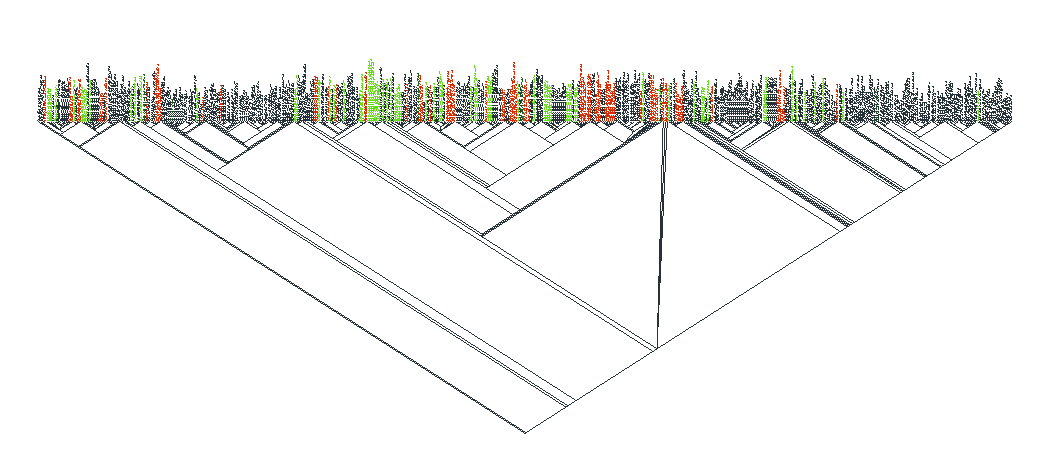
\includegraphics{figs/unnamed-chunk-8-1} 

}

\caption{Complete 476 eukaryotes tree. Green species have been filled in by a genus proxy in TimeTree. Red species have been filled in by looking at NCBI Taxonomy.}\label{fig:unnamed-chunk-8}
\end{figure}


\hypertarget{gene-selection-and-annotation}{%
\subsection{Gene selection and
annotation}\label{gene-selection-and-annotation}}

The anchoring point for this study is basic annotation about genes and
the pathways in which they participate. This section describes the
process of structuring such data. In the end we will have a table to
which all kinds of additional data will be left joined into.
\hypertarget{neurotransmitter-systems-annotation}{%
\paragraph{Neurotransmitter systems
annotation}\label{neurotransmitter-systems-annotation}}

\texttt{}\\
We start by querying the KEGG api for the pathways of interest.
Resulting data is then pivoted to a wider format.

\begin{table}[H]

\caption{\label{tab:link_pathway_entrez}All links between genes and pathways in KEGG.}
\begin{tabular}[t]{rlllll}
\toprule
\multicolumn{6}{c}{\bgroup\fontsize{12}{14}\selectfont \cellcolor[HTML]{EEEEEE}{\ttfamily{\textbf{link\_pathway\_entrez}}}\egroup{}} \\
\cmidrule(l{3pt}r{3pt}){1-6}
\# & Col. name & Col. type & Used? & Example & Description\\
\midrule
\rowcolor{gray!6}  1 & entrez\_id & character & yes & hsa:10411 & NCBI Taxonomy identifier\\
2 & pathway\_id & character & yes & path:hsa04726 & KEGG pathway ID\\
\bottomrule
\multicolumn{6}{l}{\textbf{Location: } data-raw/download/link\_pathway\_entrez.tsv}\\
\multicolumn{6}{l}{\textbf{Source: } http://rest.kegg.jp/link/pathway/hsa}\\
\end{tabular}
\end{table}

\begin{Shaded}
\begin{Highlighting}[]
\NormalTok{pathways <-}\StringTok{ }\KeywordTok{tribble}\NormalTok{(}
  \OperatorTok{~}\NormalTok{pathway_id,      }\OperatorTok{~}\NormalTok{pathway_name, }
  \StringTok{"path:hsa04724"}\NormalTok{,  }\StringTok{"glutamatergic"}\NormalTok{,}
  \StringTok{"path:hsa04725"}\NormalTok{,  }\StringTok{"cholinergic"}\NormalTok{,  }
  \StringTok{"path:hsa04726"}\NormalTok{,  }\StringTok{"serotonergic"}\NormalTok{, }
  \StringTok{"path:hsa04727"}\NormalTok{,  }\StringTok{"gabaergic"}\NormalTok{,    }
  \StringTok{"path:hsa04728"}\NormalTok{,  }\StringTok{"dopaminergic"}\NormalTok{, }
  \StringTok{"path:hsa04721"}\NormalTok{,  }\StringTok{"vesicle"}
\NormalTok{)}

\CommentTok{# removing hsa prefix}
\NormalTok{link_pathway_entrez[[}\StringTok{"entrez_id"}\NormalTok{]] }\OperatorTok\StringTok{ }\KeywordTok{str_split_n}\NormalTok{(}\StringTok{":"}\NormalTok{, }\DecValTok{2}\NormalTok{)}

\CommentTok{# filtering for pathways of interest and pivoting}
\NormalTok{gene_pathways <-}\StringTok{ }\KeywordTok{inner_join}\NormalTok{(link_pathway_entrez, pathways) }\OperatorTok
\StringTok{  }\KeywordTok{mutate}\NormalTok{(}\DataTypeTok{n =} \DecValTok{1}\NormalTok{) }\OperatorTok
\StringTok{  }\KeywordTok{pivot_wider}\NormalTok{(}
    \DataTypeTok{id_cols =}\NormalTok{ entrez_id,}
    \DataTypeTok{names_from =}\NormalTok{ pathway_name, }
    \DataTypeTok{values_from =}\NormalTok{ n,}
    \DataTypeTok{values_fn =} \KeywordTok{list}\NormalTok{(}\DataTypeTok{n =}\NormalTok{ length),}
    \DataTypeTok{values_fill =} \KeywordTok{list}\NormalTok{(}\DataTypeTok{n =} \DecValTok{0}\NormalTok{)}
\NormalTok{  ) }\OperatorTok
\StringTok{  }\CommentTok{# filling 1's in all systems for synaptic vesicle genes}
\StringTok{  }\CommentTok{# mutate_at(pathways[["pathway_name"]], ~ ifelse(vesicle == 1, 1L, .)) %>%}
\StringTok{  }\KeywordTok{mutate}\NormalTok{(}\DataTypeTok{system_count =} \KeywordTok{rowSums}\NormalTok{(}\KeywordTok{select}\NormalTok{(., }\OperatorTok{-}\NormalTok{entrez_id, }\OperatorTok{-}\NormalTok{vesicle)))}

\CommentTok{# exporting for package use}
\NormalTok{usethis}\OperatorTok{::}\KeywordTok{use_data}\NormalTok{(gene_pathways, }\DataTypeTok{overwrite =} \OtherTok{TRUE}\NormalTok{)}
\end{Highlighting}
\end{Shaded}

\begin{verbatim}
## <U+2714> Setting active project to 'C:/R/neuro'
## <U+2714> Saving 'gene_pathways' to 'data/gene_pathways.rda'
\end{verbatim}

\begin{table}[H]
\centering
\resizebox{\linewidth}{!}{
\begin{tabular}{lrrrrrrr}
\toprule
entrez\_id & vesicle & glutamatergic & cholinergic & serotonergic & gabaergic & dopaminergic & system\_count\\
\midrule
\rowcolor{gray!6}  10312 & 1 & 0 & 0 & 0 & 0 & 0 & 0\\
10497 & 1 & 0 & 0 & 0 & 0 & 0 & 0\\
\rowcolor{gray!6}  10814 & 1 & 0 & 0 & 0 & 0 & 0 & 0\\
10815 & 1 & 0 & 0 & 0 & 0 & 0 & 0\\
\rowcolor{gray!6}  112755 & 1 & 0 & 0 & 0 & 0 & 0 & 0\\
\addlinespace
1173 & 1 & 0 & 0 & 0 & 0 & 0 & 0\\
\bottomrule
\end{tabular}}
\end{table}

\hypertarget{base-id-lookup-table}{%
\paragraph{Base ID lookup table}\label{base-id-lookup-table}}

\texttt{}\\
Now we start building a base ID lookup table containing entrez gene IDs,
STRING ensembl protein IDs, ensembl gene IDs, STRING protein names and
entrez gene names. Every piece of data in subsequent analyses will be
progressively joined to it.

\begin{table}[H]

\caption{\label{tab:link_entrez_string}Conversion dictionary from entrez ID to STRING's ensembl protein ID.}
\begin{tabular}[t]{rlllll}
\toprule
\multicolumn{6}{c}{\bgroup\fontsize{12}{14}\selectfont \cellcolor[HTML]{EEEEEE}{\ttfamily{\textbf{link\_entrez\_string}}}\egroup{}} \\
\cmidrule(l{3pt}r{3pt}){1-6}
\# & Col. name & Col. type & Used? & Example & Description\\
\midrule
\rowcolor{gray!6}  1 & taxid & numeric & no & 9606 & NCBI Taxonomy ID\\
2 & entrez\_id & numeric & yes & 7157 & entrez gene ID\\
\rowcolor{gray!6}  3 & string\_id & character & yes & 9606.ENSP00000269305 & STRING ID\\
\bottomrule
\multicolumn{6}{l}{\textbf{Location: } data-raw/download/human.entrez\_2\_string.2018.tsv.gz}\\
\multicolumn{6}{l}{\textbf{Source: } https://string-db.org/mapping\_files/entrez/human.entrez\_2\_string.2018.tsv.gz}\\
\end{tabular}
\end{table}
\begin{table}[H]

\caption{\label{tab:string_names}Conversion dictionary from STRING ID to protein name.}
\begin{tabular}[t]{rlllll}
\toprule
\multicolumn{6}{c}{\bgroup\fontsize{12}{14}\selectfont \cellcolor[HTML]{EEEEEE}{\ttfamily{\textbf{string\_names}}}\egroup{}} \\
\cmidrule(l{3pt}r{3pt}){1-6}
\# & Col. name & Col. type & Used? & Example & Description\\
\midrule
\rowcolor{gray!6}  1 & taxid & numeric & no & 9606 & NCBI Taxonomy ID\\
2 & string\_name & character & yes & TP53 & protein name\\
\rowcolor{gray!6}  3 & string\_id & character & yes & 9606.ENSP00000269305 & STRING ID\\
\bottomrule
\multicolumn{6}{l}{\textbf{Location: } data-raw/download/human.name\_2\_string.tsv.gz}\\
\multicolumn{6}{l}{\textbf{Source: } https://string-db.org/mapping\_files/STRING\_display\_names/human.name\_2\_string.tsv.gz}\\
\end{tabular}
\end{table}
\begin{table}[H]

\caption{\label{tab:entrez_names}Conversion dictionary from entrez ID to gene name.}
\begin{tabular}[t]{rlllll}
\toprule
\multicolumn{6}{c}{\bgroup\fontsize{12}{14}\selectfont \cellcolor[HTML]{EEEEEE}{\ttfamily{\textbf{entrez\_names}}}\egroup{}} \\
\cmidrule(l{3pt}r{3pt}){1-6}
\# & Col. name & Col. type & Used? & Example & Description\\
\midrule
\rowcolor{gray!6}  1 & taxid & numeric & no & 9606 & taxon ID\\
2 & entrez\_id & character & yes & 7157 & entrez gene ID\\
\rowcolor{gray!6}  3 & entrez\_name & character & yes & TP53 & gene name\\
4 & ... & ... & no & ... & (too many unrelated fields)\\
\bottomrule
\multicolumn{6}{l}{\textbf{Location: } data-raw/download/Homo\_sapiens.gene\_info.gz}\\
\multicolumn{6}{l}{\textbf{Source: } https://ftp.ncbi.nlm.nih.gov/gene/DATA/GENE\_INFO/Mammalia/Homo\_sapiens.gene\_info.gz}\\
\end{tabular}
\end{table}
\begin{table}[H]

\caption{\label{tab:link_ensembl_entrez}Conversion dictionary from entrez ID to ensembl gene (ENSG) ID.}
\begin{tabular}[t]{rlllll}
\toprule
\multicolumn{6}{c}{\bgroup\fontsize{12}{14}\selectfont \cellcolor[HTML]{EEEEEE}{\ttfamily{\textbf{link\_ensembl\_entrez}}}\egroup{}} \\
\cmidrule(l{3pt}r{3pt}){1-6}
\# & Col. name & Col. type & Used? & Example & Description\\
\midrule
\rowcolor{gray!6}  1 & entrez\_id & character & yes & hsa:7157 & entrez gene ID\\
2 & ensembl\_id & character & yes & ensembl:ENSG00000141510 & ensembl gene ID\\
\bottomrule
\multicolumn{6}{l}{\textbf{Location: } data-raw/download/link\_ensembl\_entrez.tsv}\\
\multicolumn{6}{l}{\textbf{Source: } http://rest.genome.jp/link/ensembl/hsa}\\
\end{tabular}
\end{table}

\begin{Shaded}
\begin{Highlighting}[]
\CommentTok{# removing all kegg prefixes (e.g. "hsa:")}
\NormalTok{link_ensembl_entrez }\OperatorTok\StringTok{ }\KeywordTok{mutate_all}\NormalTok{(}\OperatorTok{~}\StringTok{ }\KeywordTok{str_split_n}\NormalTok{(., }\StringTok{":"}\NormalTok{, }\DecValTok{2}\NormalTok{))}

\CommentTok{# joining all data}
\NormalTok{gene_ids <-}\StringTok{ }\NormalTok{gene_pathways }\OperatorTok
\StringTok{  }\KeywordTok{select}\NormalTok{(entrez_id) }\OperatorTok
\StringTok{  }\KeywordTok{left_join}\NormalTok{(link_ensembl_entrez) }\OperatorTok
\StringTok{  }\KeywordTok{left_join}\NormalTok{(link_entrez_string) }\OperatorTok
\StringTok{  }\KeywordTok{left_join}\NormalTok{(string_names) }\OperatorTok
\StringTok{  }\KeywordTok{left_join}\NormalTok{(entrez_names)}
\end{Highlighting}
\end{Shaded}

Some STRING proteins couldn't be automatically resolved, so we perform
it manually

\begin{Shaded}
\begin{Highlighting}[]
\NormalTok{gene_ids[}\OperatorTok{!}\KeywordTok{complete.cases}\NormalTok{(gene_ids),]}
\end{Highlighting}
\end{Shaded}

\begin{tabular}{lllll}
\toprule
entrez\_id & ensembl\_id & string\_id & string\_name & entrez\_name\\
\midrule
\rowcolor{gray!6}  9296 & ENSG00000128524 & NA & NA & ATP6V1F\\
100137049 & ENSG00000243708 & NA & NA & PLA2G4B\\
\rowcolor{gray!6}  85358 & ENSG00000251322 & NA & NA & SHANK3\\
8681 & ENSG00000168970 & NA & NA & JMJD7-PLA2G4B\\
\rowcolor{gray!6}  1139 & ENSG00000175344 & NA & NA & CHRNA7\\
\addlinespace
107987478 & NA & NA & NA & LOC107987478\\
\rowcolor{gray!6}  107987479 & NA & NA & NA & LOC107987479\\
1564 & ENSG00000205702 & NA & NA & CYP2D7\\
\rowcolor{gray!6}  801 & ENSG00000198668 & NA & NA & CALM1\\
805 & ENSG00000143933 & NA & NA & CALM2\\
\addlinespace
\rowcolor{gray!6}  808 & ENSG00000160014 & NA & NA & CALM3\\
\bottomrule
\end{tabular}

\begin{Shaded}
\begin{Highlighting}[]
\NormalTok{complete_info <-}\StringTok{ }\KeywordTok{tribble}\NormalTok{(}
  \OperatorTok{~}\NormalTok{entrez_id,    }\OperatorTok{~}\NormalTok{ensembl_id,        }\OperatorTok{~}\NormalTok{string_id,              }\OperatorTok{~}\NormalTok{string_name,     }\OperatorTok{~}\NormalTok{entrez_name,  }
  \StringTok{"9296"}\NormalTok{,       }\StringTok{"ENSG00000128524"}\NormalTok{,  }\StringTok{"9606.ENSP00000417378"}\NormalTok{,  }\StringTok{"ATP6V1F"}\NormalTok{,        }\StringTok{"ATP6V1F"}\NormalTok{,      }
  \StringTok{"100137049"}\NormalTok{,  }\StringTok{"ENSG00000243708"}\NormalTok{,  }\StringTok{"9606.ENSP00000396045"}\NormalTok{,  }\StringTok{"PLA2G4B"}\NormalTok{,        }\StringTok{"PLA2G4B"}\NormalTok{,      }
  \StringTok{"85358"}\NormalTok{,      }\StringTok{"ENSG00000251322"}\NormalTok{,  }\OtherTok{NA}\NormalTok{,                      }\OtherTok{NA}\NormalTok{,               }\StringTok{"SHANK3"}\NormalTok{,       }
  \StringTok{"8681"}\NormalTok{,       }\StringTok{"ENSG00000168970"}\NormalTok{,  }\StringTok{"9606.ENSP00000371886"}\NormalTok{,  }\StringTok{"JMJD7-PLA2G4B"}\NormalTok{,  }\StringTok{"JMJD7-PLA2G4B"}\NormalTok{,}
  \StringTok{"1139"}\NormalTok{,       }\StringTok{"ENSG00000175344"}\NormalTok{,  }\StringTok{"9606.ENSP00000407546"}\NormalTok{,  }\StringTok{"CHRNA7"}\NormalTok{,         }\StringTok{"CHRNA7"}\NormalTok{,       }
  \StringTok{"107987478"}\NormalTok{,  }\OtherTok{NA}\NormalTok{,                 }\OtherTok{NA}\NormalTok{,                      }\OtherTok{NA}\NormalTok{,               }\StringTok{"LOC107987478"}\NormalTok{, }
  \StringTok{"107987479"}\NormalTok{,  }\OtherTok{NA}\NormalTok{,                 }\OtherTok{NA}\NormalTok{,                      }\OtherTok{NA}\NormalTok{,               }\StringTok{"LOC107987479"}\NormalTok{, }
  \StringTok{"1564"}\NormalTok{,       }\StringTok{"ENSG00000205702"}\NormalTok{,  }\OtherTok{NA}\NormalTok{,                      }\OtherTok{NA}\NormalTok{,               }\StringTok{"CYP2D7"}\NormalTok{,       }
  \StringTok{"801"}\NormalTok{,        }\StringTok{"ENSG00000198668"}\NormalTok{,  }\StringTok{"9606.ENSP00000349467"}\NormalTok{,  }\StringTok{"CALM1"}\NormalTok{,          }\StringTok{"CALM1"}\NormalTok{,        }
  \StringTok{"805"}\NormalTok{,        }\StringTok{"ENSG00000143933"}\NormalTok{,  }\StringTok{"9606.ENSP00000272298"}\NormalTok{,  }\StringTok{"CALM2"}\NormalTok{,          }\StringTok{"CALM2"}\NormalTok{,        }
  \StringTok{"808"}\NormalTok{,        }\StringTok{"ENSG00000160014"}\NormalTok{,  }\StringTok{"9606.ENSP00000291295"}\NormalTok{,  }\StringTok{"CALM3"}\NormalTok{,          }\StringTok{"CALM3"}
\NormalTok{)}

\CommentTok{# removing incomplete cases and adding updated ones}
\NormalTok{gene_ids }\OperatorTok\StringTok{ }\NormalTok{na.omit }\OperatorTok\StringTok{ }\KeywordTok{bind_rows}\NormalTok{(complete_info)}

\CommentTok{# removing taxid prefix from STRING IDs}
\NormalTok{gene_ids[[}\StringTok{"string_id"}\NormalTok{]] }\OperatorTok\StringTok{ }\KeywordTok{str_split_n}\NormalTok{(}\StringTok{"}\CharTok{\textbackslash{}\textbackslash{}}\StringTok{."}\NormalTok{, }\DecValTok{2}\NormalTok{)}

\CommentTok{# exporting for package use}
\NormalTok{usethis}\OperatorTok{::}\KeywordTok{use_data}\NormalTok{(gene_ids, }\DataTypeTok{overwrite =} \OtherTok{TRUE}\NormalTok{)}
\end{Highlighting}
\end{Shaded}

\begin{verbatim}
## <U+2714> Saving 'gene_ids' to 'data/gene_ids.rda'
\end{verbatim}


\hypertarget{neuroexclusivity}{%
\subsection{Neuroexclusivity}\label{neuroexclusivity}}

Explanation

\hypertarget{expression}{%
\subsubsection{Expression}\label{expression}}

\hypertarget{pathways}{%
\subsubsection{Pathways}\label{pathways}}

\hypertarget{cog-data}{%
\subsection{COG data}\label{cog-data}}

\hypertarget{network}{%
\subsection{Network}\label{network}}

\hypertarget{analysis}{%
\section{Analysis}\label{analysis}}

Analysis

\begin{Shaded}
\begin{Highlighting}[]
\CommentTok{#leave this chunk}
\end{Highlighting}
\end{Shaded}

\end{document}
